\documentclass[12pt, oneside]{article}   	% use "amsart" instead of "article" for AMSLaTeX format
\usepackage[margin=1in]{geometry}                		% See geometry.pdf to learn the layout options. There are lots.
\geometry{letterpaper}                   		% ... or a4paper or a5paper or ... 
\usepackage{graphicx}				% Use pdf, png, jpg, or eps§ with pdflatex; use eps in DVI mode

								% TeX will automatically convert eps --> pdf in pdflatex		
\usepackage{amssymb}
\usepackage{siunitx}
\usepackage{physics}

\usepackage{color}
\usepackage{titling}
\usepackage[T1]{fontenc}
\usepackage{mathtools}  % loads »amsmath«
\usepackage{cancel}
\usepackage{physics}
\usepackage{hyperref}
\usepackage{color}
%SetFonts
\newcommand\Rey{\mbox{\textit{Re}}}
\renewcommand{\thefootnote}{\fnsymbol{footnote}}

\title{\vspace{-6ex} \large PHYS 516- METHODS OF COMPUTATIONAL PHYSICS \\
        \normalsize ASSIGNMENT 2- MONTE CARLO BASICS }
\author{\vspace{-3ex}Anup V Kanale}
\date{\vspace{-2ex} \today}

\begin{document}
\maketitle
\section{Programming: Testing the Central Theorem of Monte Carlo Estimate}
In this assignment, the dependence of Monte Carlo (MC) error is numerically tested on the sample size M.
	\begin{equation}
	Std\{\overline{f(x)}\} = \frac{Std\{f(x)\}}{\sqrt{M}}
	\end{equation}
Mean integral of $\pi$ is used as the sample.
	\begin{equation}
	\frac{1}{M} \sum\limits_{i=1}^{M} \frac{4}{1+r_n^2} = \overline{\frac{4}{1+r_n^2}} \approx \pi (r_n \in \left[0,1 \right]) 
	\end{equation}
The plot below shows the estimate of $\pi$ as a function of the number of Monte Carlo trials.
 \subsection{Monte Carlo Estimate}
 The MC estimate of $\pi$ is calculated, along with the error, using different number of trials and the results are shown in the plot below. The unbiased estimate of the standard deviation is given by
	\begin{equation}
	SD = \sqrt{\frac{\overline{f^2} - (\overline{f})^2}{M-1}}
	\end{equation}
 	\begin{figure} [!htbp]
	\centering
	 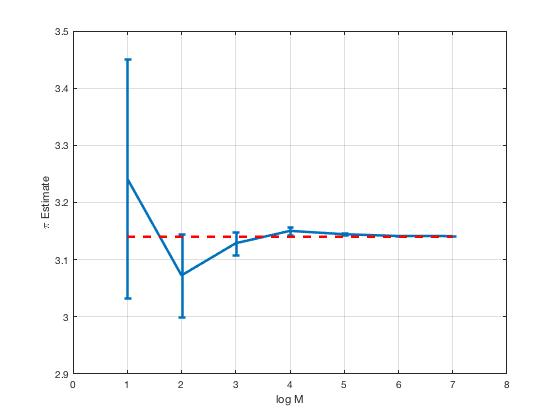
\includegraphics[scale=0.35]{MC_piEstimate.jpg}
	\caption{Monte Carlo Estimation of Pi}
	\end{figure}
	
	It is easily seen that the error decreases with increasing number of trials, and that beyond $10^5$ trials, increasing $M$ has negligible effect on the error.	
	\begin{figure} [!htbp]
	\centering
	 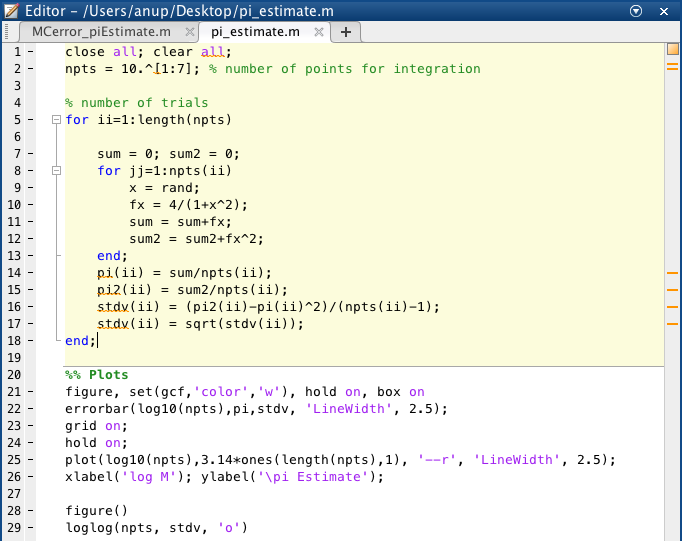
\includegraphics[scale=0.5]{pi_MCestimate_code.jpg}
	\caption{Source Code}
	\end{figure}
\subsection{Monte Carlo Error}
We next perform a numerical experiment to directly measure the standard deviation of the MC estimate. To do so, for each of the above M values, $\pi$ is estimated $N_{seed}$ times using $N_{seed}$ different random-number seeds. The standard deviation $\sigma_M$ of these $N_{seed}$ estimates $\pi_1$, $\pi_2$, ..., $\pi_{N_{seed}}$
	\begin{equation}
	\sigma_M = \sqrt{\frac{1}{N_{seed}} \sum\limits_{i=1}^{N_{seed}} \pi_i^2 - \left[ \frac{1}{N_{seed}}\sum\limits_{i=1}^{N_{seed}} \pi_i\right]^2 }
	\end{equation}
The measured values of $\log_{10} \sigma_M$ are shown as a function of $\log_{10} M$ in the plot below. If the MC error decreases as $\sigma_M = C/\sqrt{M}$, then  
$$log_{10}\sigma_M = log_{10}C - \frac{1}{2} log_{10}M $$
Using a least square fit, the equation of the line obtained is
 $$log_{10}\sigma_M = -0.1653 - 0.505 log_{10}M $$
We see that the unbiased estimates from the previous question neatly fall onto this fitted line.
 	\begin{figure} [!htbp]
	\centering
	 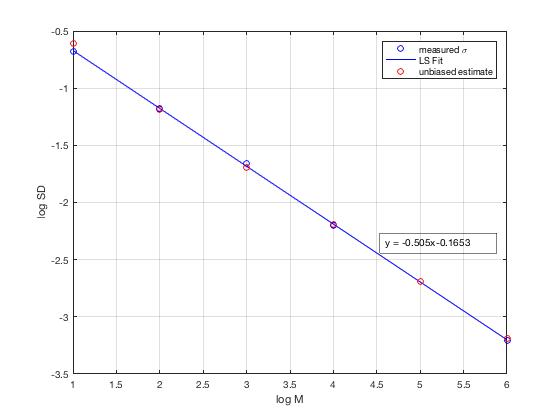
\includegraphics[scale=0.5]{stdv_fit.jpg}
	\caption{Unbiased Estimates and Measured values of Standard Deviation}
	\end{figure}
	
		\begin{figure} [!htbp]
	\centering
	 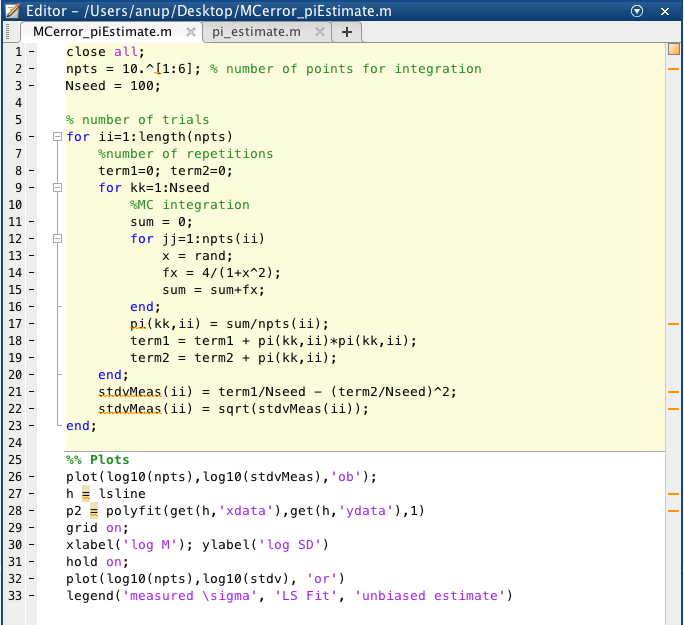
\includegraphics[scale=0.5]{stdv_fitCode.jpg}
	\caption{Source Code}
	\end{figure}
\pagebreak
\section{Non-uniform random number generation: Box-Muller Transformation}
A Box-Muller algorithm generates a normally distributed random number. This algorithm is similar in principle to the Greenland Phenomenon.

First a set of independent uniform random numbers $r_1$ and $r_2$ are generated in the range $(0,1)$.  The following transformations are then applied to get two new independent random numbers.
	\begin{align}
	\zeta_1 &= \sqrt{-2 \ln r_1} \cos{(2 \pi r_2)} \\
	\zeta_2 &= \sqrt{-2 \ln r_1} \sin{(2 \pi r_2)} 
	\end{align}
Now let us try to express $r_1$ and $r_2$ in terms of $\zeta_1$ and $\zeta_2$. Summing and squaring Eq(5) and (6),
	\begin{align}
	\therefore \zeta_1 ^2 + \zeta_2 ^2 &= -2 \ln{r_1} \\
	\implies r_1 &= \exp{-\frac{\zeta_1 ^2 + \zeta_2 ^2}{2}}
	\end{align}
Similarly, dividing Eq.(6) by Eq.(5),
	\begin{equation}
	r_2 = \frac{1}{2\pi} \tan^{-1}{\left( \frac{\zeta_2}{\zeta_1} \right) }
	\end{equation}
In a given area, the number of samples is preserved, i.e.,
	$$N P(r_1,r_2)dr_1 dr_2 = N  P'(\zeta_1, \zeta_2) S(r_1, r_2, \zeta_1,\zeta_2) $$
The new transformed area can be expressed as
	$$ S = \left| \left| \pdv{(\zeta_1, \zeta_2)}{(r_1, r_2)} \right| \right| dr_1 dr_2$$
The probability of finding a point in the $(r_1,r_2)$ space is 1, since the distribution is uniform. Using this fact, and the above two equations we can write
	\begin{align}
		 P'(\zeta_1, \zeta_2) &=\left| \left| \pdv{(\zeta_1, \zeta_2)}{(r_1, r_2)} \right| \right| ^{-1} \underbrace{P(r_1,r_2)}_{\text =1} \\
		 & = \underbrace{\left| \left| \pdv{(r_1, r_2)}{(\zeta_1, \zeta_2)} \right| \right|}_{J}
		 \end{align}
The determinant in Eq.(11) is known as the Jacobian and is is evaluated as follows:
	\begin{align}
		 J = \left| \begin{vmatrix}
		 \pdv{r_1}{\zeta_1} & \pdv{r_1}{\zeta_2} \\
		 \pdv{r_2}{\zeta_1} & \pdv{r_2}{\zeta_2}
		 \end{vmatrix} \right|	 = \left| \pdv{r_1}{\zeta_1} \pdv{r_2}{\zeta_2} - \pdv{r_2}{\zeta_1} \pdv{r_1}{\zeta_2} \right|
	\end{align}
Let us now calculate the terms in the Jacobian using Eq.(8) and Eq.(9),
	\begin{align}
	\pdv{r_1}{\zeta_1} &= -\zeta_1 \exp{-\frac{\zeta_1 ^2 + \zeta_2 ^2}{2}} = -\zeta_1 r_1 \\
	\pdv{r_1}{\zeta_2} &= -\zeta_2 \exp{-\frac{\zeta_1 ^2 + \zeta_2 ^2}{2}} = -\zeta_2 r_1 \\
	\pdv{r_2}{\zeta_1} &= -\frac{\zeta_2}{2\pi(\zeta_1 ^2 + \zeta_2 ^2)} \\
	\pdv{r_2}{\zeta_2} &=  \frac{\zeta_1}{2\pi(\zeta_1 ^2 + \zeta_2 ^2)}
	\end{align}
Substituting these in Eq. (11)
	\begin{align} 
	 P'(\zeta_1, \zeta_2) &= \left| -\frac{\zeta_1^2 r_1}{2\pi(\zeta_1 ^2 + \zeta_2 ^2)} -\frac{\zeta_2^2 r_1}{2\pi(\zeta_1 ^2 + \zeta_2 ^2)} \right| \\
	&= \frac{r_1}{2 \pi} \\
	&= \frac{1}{2\pi} \exp{\zeta_1 ^2 + \zeta_2 ^2} \\
	&= \sqrt{\frac{1}{2\pi}} \exp{\zeta_1 ^2} \sqrt{\frac{1}{2\pi}} \exp{\zeta_2 ^2} \\
	\therefore P'(\zeta_1, \zeta_2) &= P'(\zeta_1) P'(\zeta_2)
	\end{align}
which means that the two variables are uncorrelated. Therefore, a general Gaussian random number distribution can be expressed as 
$$ P'(\zeta) = \sqrt{\frac{1}{2\pi}} \exp{\zeta ^2} $$
	\begin{figure} [!htbp]
	 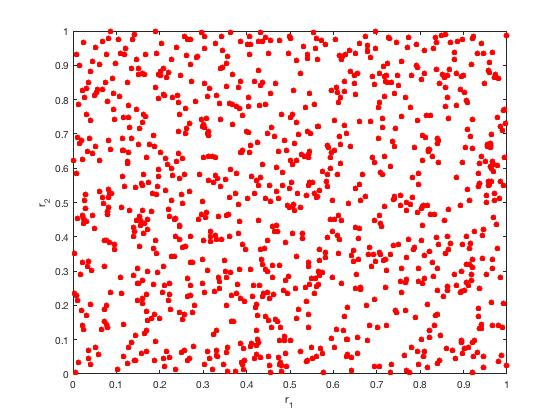
\includegraphics[scale=0.40]{r1r2_space.jpg}
	 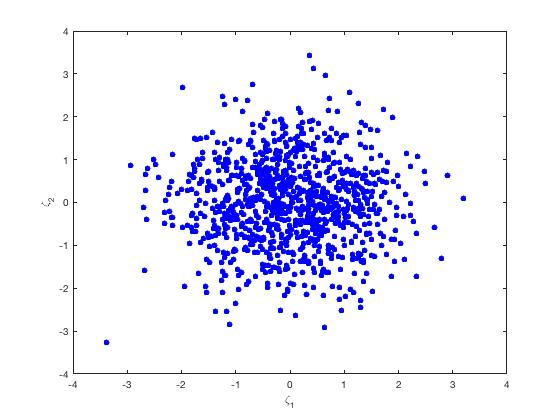
\includegraphics[scale=0.40]{zeta1zeta2_space.jpg}
	\caption{$r_1-r_2$ space and the transformed $\zeta_1-\zeta_2$ space}
	\end{figure}

	\begin{figure} [!htbp]
	\centering
	 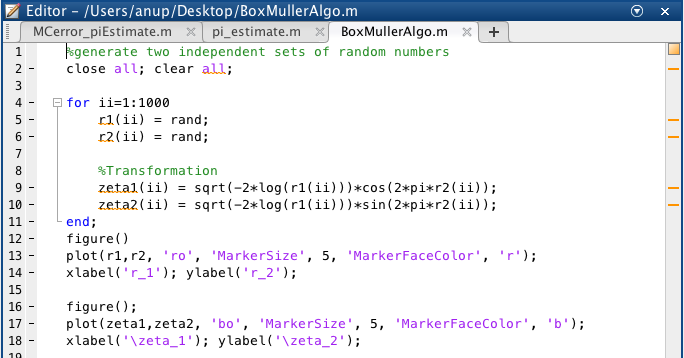
\includegraphics[scale=0.6]{BoxMullerAlgo_code.jpg}
	\caption{Source Code}
	\end{figure}
\end{document}